% !TeX root = ..\main.tex
\pagestyle{fancy-style}
\npchapter{Einleitung} \label{ch:introduction}
\pagenumbering{arabic}
Dieses Kapitel führt in das zu erforschende Thema ein. Darüber hinaus wird die Motivation zur Evaluation von Bun dargelegt. Zusätzlich werden die Ziele und der Aufbau der Arbeit näher betrachtet.

\section{Motivation} \label{sec:introduction-motivation}
JavaScript ist aktuell eine beliebte Programmiersprache. In einer Umfrage unter Entwicklern auf Stack Overflow, an der mehr als 89.000 Entwickler teilgenommen haben, wird JavaScript zum elften Jahr in Folge als die am häufigsten verwendete Programmiersprache identifiziert. Mehr als 63\% der befragten Entwickler haben JavaScript als ihre favorisierte Technologie angegeben. Unter den professionellen Entwicklern liegt der Anteil mit 65\% höher. Zusätzlich ist TypeScript, eine stark typisierte Programmiersprache, die auf JavaScript aufbaut, ebenfalls verbreitet \cite{Microsoft.o.J.}. Etwa 39\% aller Entwickler und ungefähr 44\% der professionellen Entwickler nutzen TypeScript. Somit ist TypeScript die viertbeliebteste Programmiersprache. Dies unterstreicht die hohe Relevanz des JavaScript-Ökosystems.\cite{StackOverflow.2023}\newline
JavaScript wird vor allem im Kontext der Web-Entwicklung verwendet \cite{Brown.2020}. Darüber hinaus nutzen etwa 3\% der weltweit bekannten Server eine Laufzeitumgebung, die JavaScript ausführen kann \cite{QSuccess.2023}. Demnach wird die Programmiersprache nicht nur für die Entwicklung im Frontend, sondern auch im Backend eingesetzt.\\

\begin{figure}[h]
	\centering
	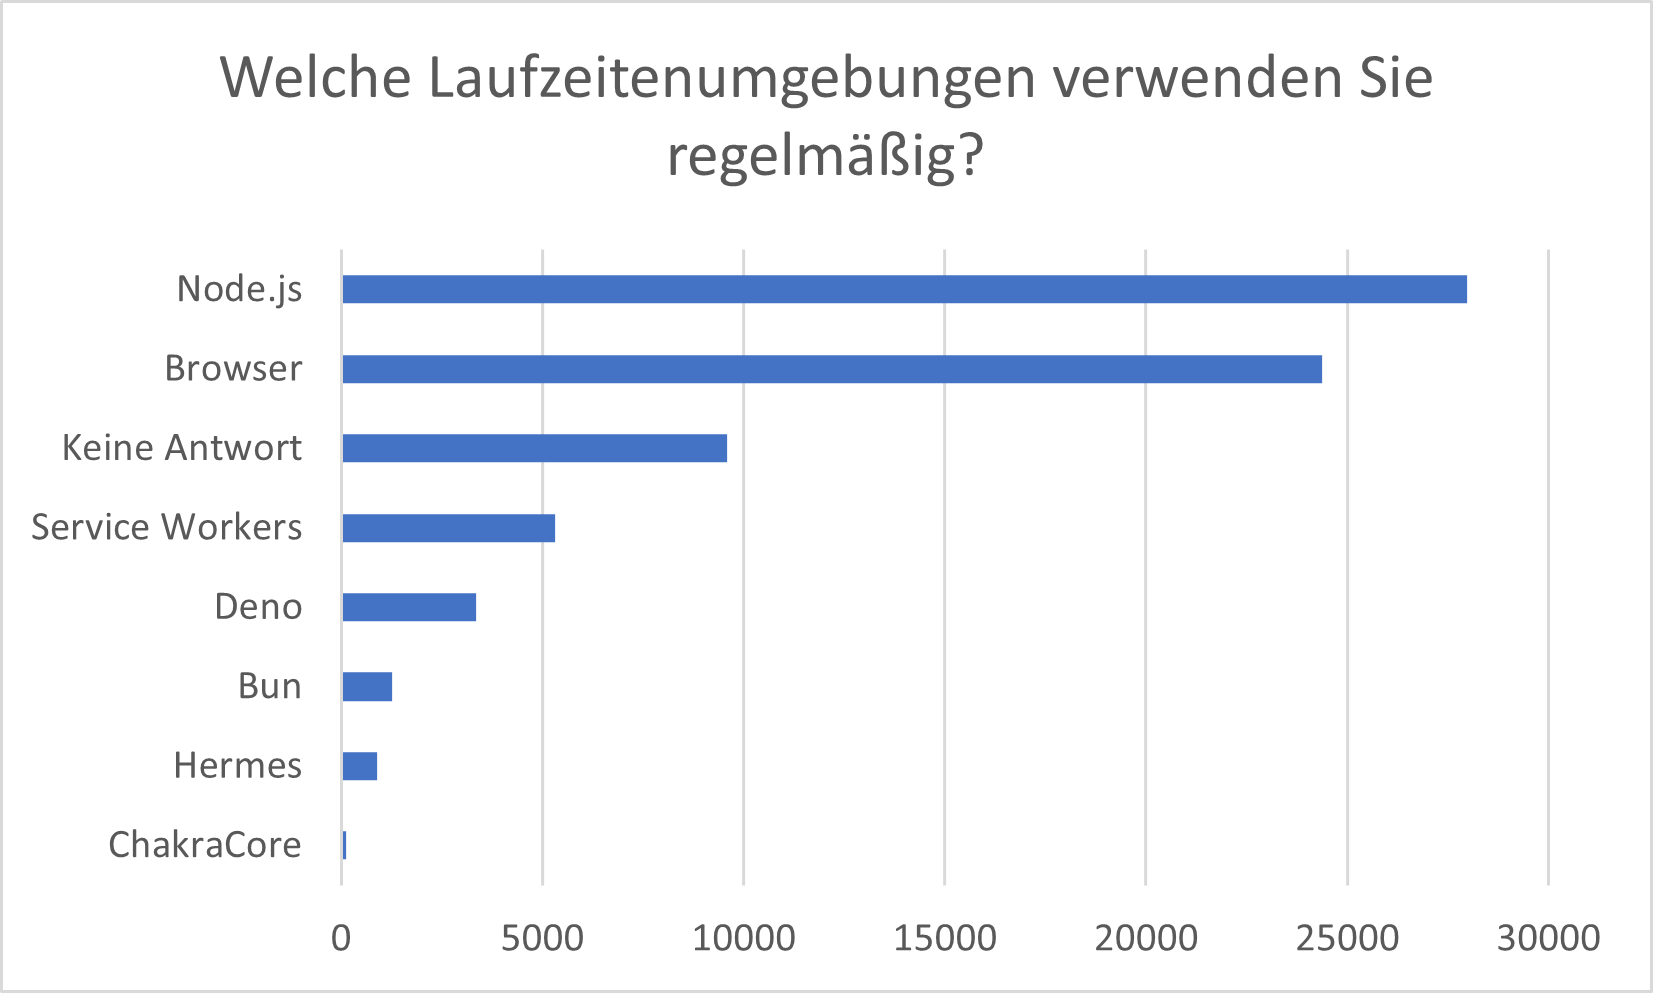
\includegraphics[width=\linewidth]{./images/WhichRuntimesDoYouUseRegularly}
	\caption{Nutzungsstatistik von JavaScript-Laufzeitumgebungen}
	\label{fig:runtime-share}
	\textit{Quelle: in Anlehnung an \cite{Greif.2022}}
\end{figure}

\noindent
\autoref{fig:runtime-share} zeigt, dass Node.js die am weitesten verbreitete Laufzeitumgebung ist. In der Umfrage \glqq State of JavaScript 2022\grqq{} gaben ca. 71\% der 30.000 befragten Entwickler an, dass sie Node.js regelmäßig als Laufzeitumgebung verwenden \cite{Greif.2022}. Dennoch erscheinen immer wieder neue Laufzeitumgebungen, die versuchen, Node.js zu verdrängen. Die neuste Alternative ist Bun, das am 9. September 2023 in der Version 1.0 veröffentlicht wurde \cite{Sumner.2023c}. In der zuvor erwähnten Umfrage haben etwa 3\% der Entwickler angegeben, dass sie Bun als eine Alternative zu Node.js verwenden, obwohl sich Bun zu diesem Zeitpunkt noch im Entwicklungsstadium befunden hat \cite{Greif.2022}.\\

\noindent
Die Entwickler von Bun werben mit Features wie erheblicher Leistungssteigerung, eleganten Schnittstellen und einer angenehmen Entwicklererfahrung \cite{OvenSh.2023b}. Die Laufzeitumgebung inkludiert einen integrierten Paketmanager, einen Bundler, eine Test-Bibliothek und einen Transpiler zum Ausführen von TypeScript. Bun besitzt das Ziel, ein Eins-zu-Eins-Ersatz für Node.js zu sein. Das heißt, Bun soll mit wenig Migrationsaufwand für alle bestehenden Node.js-Projekte verwendet werden können und wird demnach für dieselben Projekte wie Node.js verwendet.\cite{Sumner.2023c}

\section{Zielsetzung} \label{sec:introduction-target}
Das Hauptziel dieser Arbeit besteht darin, die Version 1.0 von Bun einer eingehenden Evaluierung zu unterziehen. Konkret wird untersucht, ob die in den Ankündigungen versprochene signifikante Leistungssteigerung im Vergleich zu Node.js tatsächlich existiert und reproduzierbar ist. Darüber hinaus wird geprüft, inwiefern bestehende Projekte auf der Basis von Node.js mit Bun kompatibel sind. Die Ergebnisse dieser Arbeit können Entwicklern bei der Entscheidung helfen, ob sie auf Bun 1.0 migrieren sollten, und sie dabei unterstützen, die Leistung ihrer bestehenden Projekte zu verbessern. Insgesamt zielt diese Untersuchung darauf ab, Klarheit über die Versprechungen von Bun 1.0 zu schaffen und Entwicklern fundierte Informationen für ihre Entscheidungsfindung zur Verfügung zu stellen. Dies spiegelt sich in den folgenden Leitfragen wider:
\begin{itemize}
    \item Welche konkreten Leistungsverbesserungen können in Bun 1.0 im Vergleich zu Node.js 18 und 21 festgestellt werden, und wie lassen sie sich quantifizieren?
    \item Inwiefern sind Node.js-Projekte kompatibel mit Bun? Wie schwierig gestaltet sich die Migration?
    \item Welche Herausforderungen und Vorteile ergeben sich bei der Verwendung von Bun 1.0 im Vergleich zu Node.js für Entwickler und Projekte?
\end{itemize}

\section{Aufbau der Arbeit} \label{sec:introduction-overview}
Im folgenden Kapitel vermittelt die Arbeit alle notwendigen theoretischen Grundlagen, die zum Verständnis des Themas notwendig sind. Dafür werden Node.js und Bun detailliert betrachtet. Des Weiteren wird Performance als Qualitätsattribut von Software definiert, um Rückschlüsse für die Performanceanalyse zu ermöglichen.\\

\noindent
Das dritte Kapitel vergleicht die Performance von Bun und Node.js in ausgewählten Testszenarien. Hierzu werden zuerst die Vorgehensweise, der Versuchsaufbau und die Implementierungen vorgestellt. Im Anschluss daran folgt die Präsentation der Ergebnisse und ein zusammenfassendes Fazit.\\

\noindent
Das vierte Kapitel setzt den Fokus auf die Kompatibilität von Projekten auf Basis von Node.js. Die Betrachtung beschränkt sich auf die Frameworks Express und Nest. Um die Kompatibilität bewerten zu können, wird pro Framework eine Anwendung beispielhaft migriert. Abschließend folgt die Bewertung der Ergebnisse in einem Fazit.\\

\noindent
Das letzte Kapitel fasst die Kernaussagen der Arbeit zusammen und prüft sie vor dem Hintergrund der zuvor definierten Ziele. Abschließend wird in einem Ausblick dargelegt, welche ergänzenden Forschungsthemen verbleiben und welchen zukünftigen Nutzen die Ergebnisse mit sich bringen.